% !TeX spellcheck = en_US
\documentclass[french]{article}
\usepackage[T1]{fontenc}
\usepackage[utf8]{inputenc}
\usepackage{lmodern}
\usepackage[a4paper]{geometry}
\usepackage{babel}
\usepackage{graphicx}

\begin{document}
\title{Nuages de points et modélisation 3D\\
TP 4 : Rendering}
\author{Marius Dufraisse}
\date{}

\maketitle

The program is to be called like this \texttt{python3 MVA\_{}NPM\_{}TP\_{}4.py}. In this setting it will display the provided normal map and then render it using the Cook-Torrance BRDF model (for result Figure \ref{fig:cook}).

\begin{figure}[h]
	\centering
	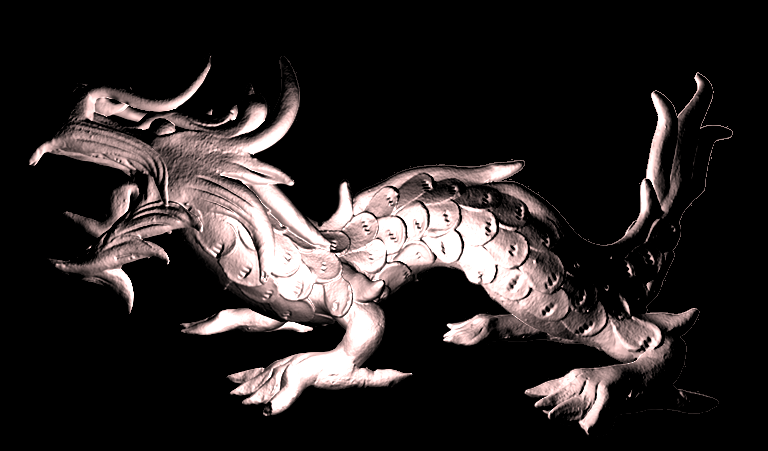
\includegraphics[width=0.6\linewidth]{render-cook.png}
	\caption{Image rendered using the Cook-Torrance model.}
	\label{fig:cook}
\end{figure}

The material model to use can be select using the option \texttt{-c} for Cook-Torrance, \texttt{-b} for Blinn-Phong (see Figure \ref{fig:blinn}) and \texttt{-l} for Lambert (see Figure \ref{fig:lambert}).

\begin{figure}[h]
	\centering
	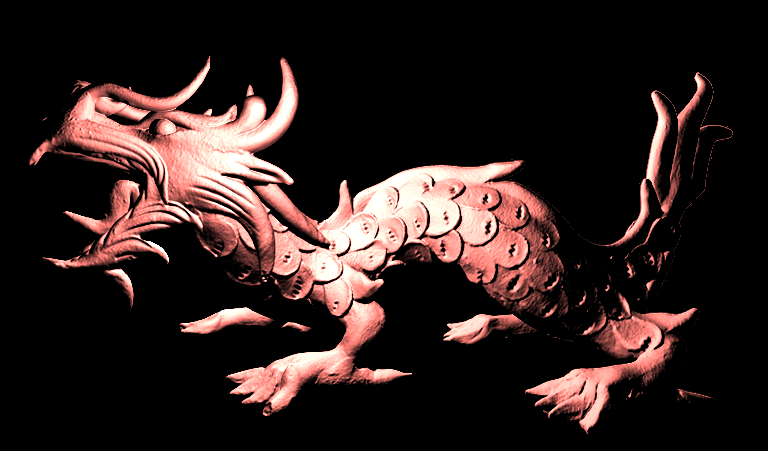
\includegraphics[width=0.6\linewidth]{render-blinn.png}
	\caption{Image rendered using the Blinn-Phong model.}
	\label{fig:blinn}
\end{figure}

\begin{figure}[h]
	\centering
	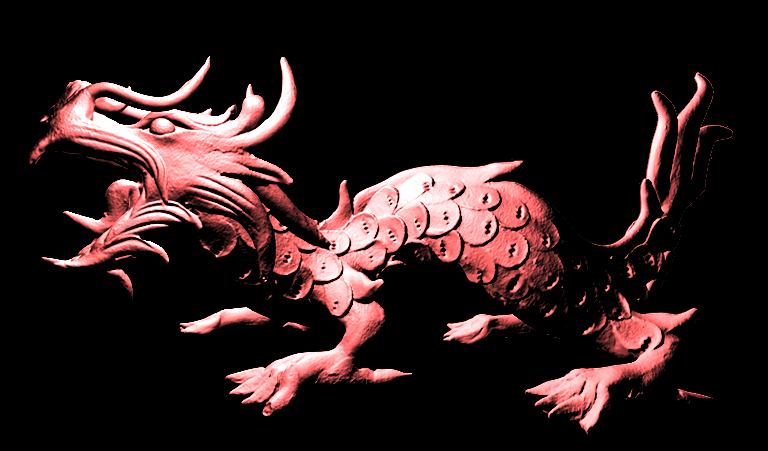
\includegraphics[width=0.6\linewidth]{render-lambert.png}
	\caption{Image rendered using the Lambert model.}
	\label{fig:lambert}
\end{figure}

I added an interactive mode that allow the user to place light sources, it is enabled using the option \texttt{-m interactif}. The code can also generate a video with moving lights, it is enabled using the option \texttt{-m video} but it does not work very well.



\end{document}
